\documentclass{article}

\usepackage{pgfplots}

\pgfplotsset{compat=1.9}

% \usetikzlibrary{}
\usepgfplotslibrary{fillbetween}

\usepackage{pgfplotstable}
\usepackage{booktabs}
\usepackage{array}
\usepackage{colortbl}

\begin{document}

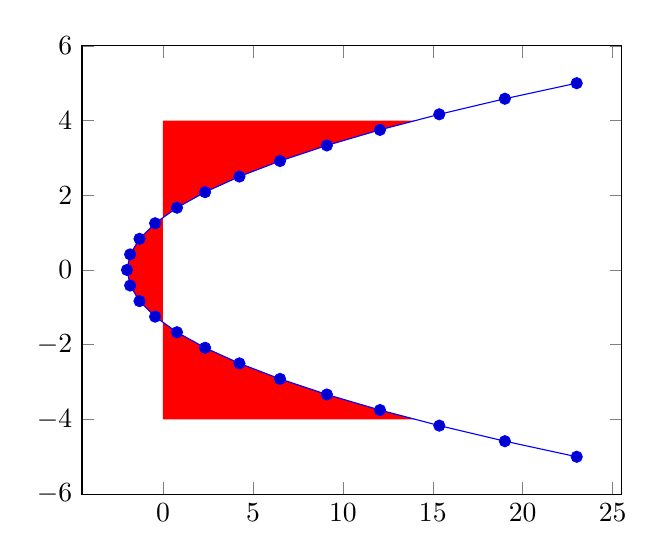
\begin{tikzpicture}
	\begin{axis}
	\addplot+[name path=A] (x^2-2,x);

	\path[name path=B] (axis cs:0,\pgfkeysvalueof{/pgfplots/ymin}) -- (axis cs:0,\pgfkeysvalueof{/pgfplots/ymax});

	\addplot fill between[of=A and B,reverse=false,soft clip={domain y=-4:4}];
	\end{axis}
\end{tikzpicture}

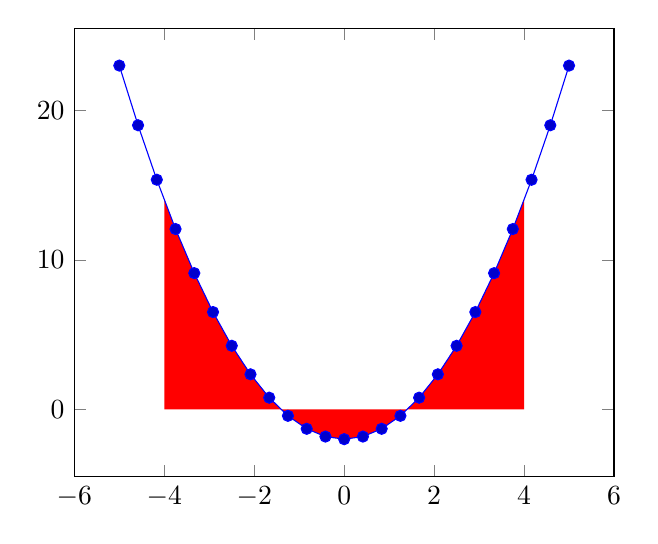
\begin{tikzpicture}
	\begin{axis}
	\addplot+[name path=A] {x^2-2};

	\path[name path=xaxis] (axis cs:-5,0) -- (axis cs:5,0);

	\addplot fill between[of=A and xaxis,soft clip={domain=-4:4}];
	\end{axis}
\end{tikzpicture}
\end{document}

